\section{What should the runtime remember?}
\label{sec:runtime}

Hybrid state lets the runtime keep observed command outcomes while the
model maintains hypotheses and pending work
(Figure~\ref{fig:runtime-written}). Its value depends on what the runtime
records: which file was seen differs from what changed and which commands
followed.

% Adapted from the repository's original state-ownership diagram.
\begin{figure}[tbp]
\centering
\resizebox{\linewidth}{!}{%
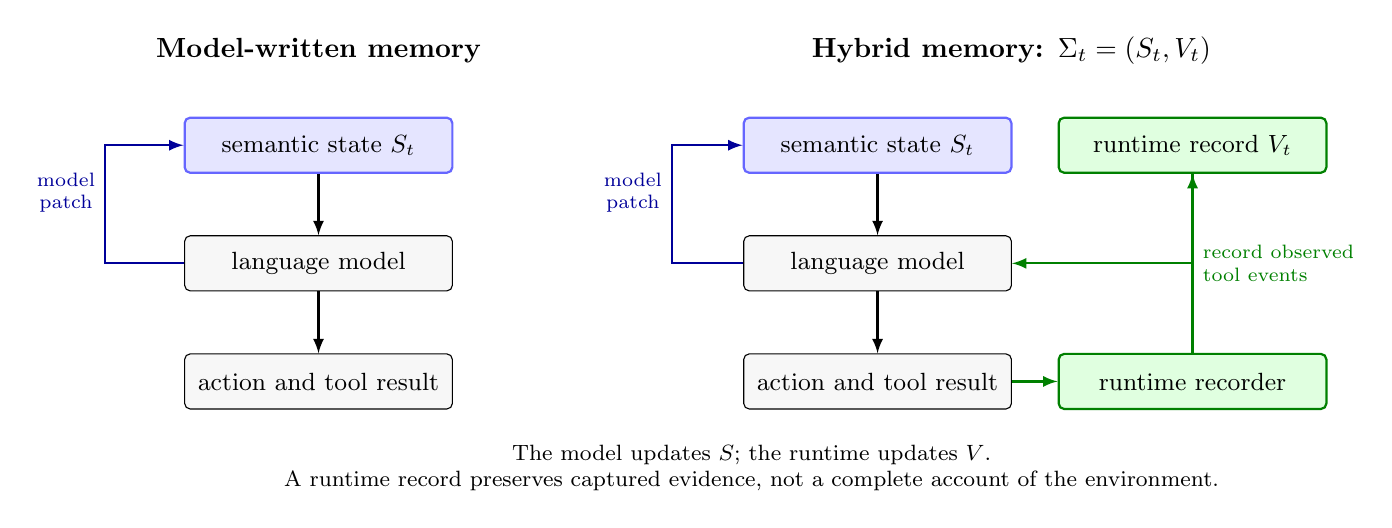
\begin{tikzpicture}[
font=\small,
box/.style={draw,rounded corners=2pt,minimum width=3.4cm,minimum height=.7cm,align=center,inner sep=3pt},
state/.style={box,fill=blue!10,draw=blue!60,thick},
record/.style={box,fill=green!12,draw=green!50!black,thick},
plain/.style={box,fill=black!3},
arr/.style={-latex,thick}]
\node[font=\bfseries] at (0,3.5) {Model-written memory};
\node[state] (s1) at (0,2.3) {semantic state $S_t$};
\node[plain] (m1) at (0,.8) {language model};
\node[plain] (a1) at (0,-.7) {action and tool result};
\draw[arr] (s1)--(m1);
\draw[arr] (m1)--(a1);
\draw[arr,blue!60!black] (m1.west)--++(-1,0)|-(s1.west)
node[pos=.3,left,font=\scriptsize,align=center]{model\\patch};
\begin{scope}[xshift=7.1cm]
\node[font=\bfseries] at (1.7,3.5) {Hybrid memory: $\Sigma_t=(S_t,V_t)$};
\node[state] (s2) at (0,2.3) {semantic state $S_t$};
\node[record] (v2) at (4,2.3) {runtime record $V_t$};
\node[plain] (m2) at (0,.8) {language model};
\node[plain] (a2) at (0,-.7) {action and tool result};
\node[record] (rec) at (4,-.7) {runtime recorder};
\draw[arr] (s2)--(m2);
\draw[arr,green!50!black] (v2.south)|-(m2.east);
\draw[arr] (m2)--(a2);
\draw[arr,blue!60!black] (m2.west)--++(-.9,0)|-(s2.west)
node[pos=.3,left,font=\scriptsize,align=center]{model\\patch};
\draw[arr,green!50!black] (a2)--(rec);
\draw[arr,green!50!black] (rec)--(v2)
node[midway,right,font=\scriptsize,align=left]{record observed\\tool events};
\end{scope}
\node[font=\footnotesize,align=center] at (5.5,-1.8)
{The model updates $S$; the runtime updates $V$.\\A runtime record preserves captured evidence, not a complete account of the environment.};
\end{tikzpicture}}
\caption{State ownership. Hybrid memory retains model-written semantic content and adds runtime-derived records. Recording an event does not establish that an extracted interpretation is correct or that all relevant events were captured.}
\label{fig:runtime-written}
\end{figure}


\subsection{From file references to execution evidence}

File references alone reach \ExploreFilesRate\% solved
(Table~\ref{tab:composition}). Adding modifications and command records
raises this to \ExploreCommandsRate\%, lowers median output from
\ExploreFilesOutputMedian{} to \ExploreCommandsOutputMedian{} thousand
tokens, and lowers median cost from \$\ExploreFilesCostMedian{} to
\$\ExploreCommandsCostMedian{}. Diagnostics, environment, and tests give
\ExploreRichRate\%; failed-attempt records give \ExploreFailuresRate\%.
None reaches full history at \ExploreControlRate\%. The gain sits between
file references and execution records; further enrichment plateaus
(Figure~\ref{fig:composition}). Rows change bundles of records, so no
single component is isolated.

\begin{table}[htbp]
\centering\small
\caption{Runtime-record contents under the same semantic schema
(exploratory, one repetition). Top: quality panel over all retained
outcomes. Bottom: resource panel, per-execution medians. Rows beginning
with $+$ add to the preceding row.}
\label{tab:composition}
\resizebox{\linewidth}{!}{\input{tables/new-composition}}

\medskip
\resizebox{\linewidth}{!}{\input{tables/new-composition-resources}}
\end{table}

% Descriptive component comparison; not an independent replication.
\begin{figure}[tbp]
\centering
\begin{tikzpicture}
\begin{axis}[
width=.47\linewidth,height=5.4cm,
title={Task success},title style={font=\small},
ylabel={Solved rate (\%)},ymin=20,ymax=60,
xmin=-.4,xmax=3.4,xtick={0,1,2,3},
xticklabels={{File\\references},{+ action\\records},{+ context\\records},{+ failure\\records}},
xticklabel style={font=\scriptsize,align=center},yticklabel style={font=\scriptsize},
label style={font=\small},grid=major,grid style={black!12},
legend style={font=\scriptsize,at={(.03,.97)},anchor=north west,draw=none,fill=white}]
\addplot[only marks,mark=*,mark size=2.5pt,blue!65!black]
table[col sep=comma,x=order,y=solved_pct]{../paper/generated/new-composition.csv};
\addlegendentry{Hybrid memory}
\addplot[dashed,black!65,domain=-.4:3.4] {\ExploreControlRate};
\addlegendentry{Full history}
\end{axis}
\begin{axis}[
at={(.52\linewidth,0)},anchor=south west,
width=.47\linewidth,height=5.4cm,
title={Cost efficiency},title style={font=\small},
ylabel={Solved/\$},ymin=10,ymax=26,
xmin=-.4,xmax=3.4,xtick={0,1,2,3},
xticklabels={{File\\references},{+ action\\records},{+ context\\records},{+ failure\\records}},
xticklabel style={font=\scriptsize,align=center},yticklabel style={font=\scriptsize},
label style={font=\small},grid=major,grid style={black!12}]
\addplot[only marks,mark=square*,mark size=2.5pt,green!45!black]
table[col sep=comma,x=order,y=solved_per_dollar]{../paper/generated/new-composition.csv};
\addplot[dashed,black!65,domain=-.4:3.4] {\ExploreControlSolvedPerDollar};
\end{axis}
\end{tikzpicture}
\caption{Exploratory comparison of cumulative runtime-owned information. Each
position adds records to the preceding configuration: action records cover
file changes and commands; context records cover diagnostics, environment,
and tests. Efficiency
includes the cost of unsuccessful episodes. Dashed lines show the same
full-history reference. These descriptive observations share their richer
configurations and reference with the first repeat of the final comparison;
they do not isolate individual components or establish a monotonic benefit.}
\label{fig:composition}
\end{figure}


Every runtime-record configuration has a lower cache hit than full history
(\ExploreCommandsCacheHitMedian--\ExploreFilesCacheHitMedian\% against
\ExploreControlCacheHitMedian\%), consistent with a changing state block
breaking prefix reuse that a growing transcript keeps. Successes per dollar rise
from \ExploreFilesSolvedPerDollar{} to \ExploreCommandsSolvedPerDollar{},
approaching but not exceeding the control's
\ExploreControlSolvedPerDollar{}. On tasks solved by every configuration,
the richest variants cost \ExploreRichFixedCostRatio{} and
\ExploreFailuresFixedCostRatio{} times full history
(Supplementary~\ref{app:composition}): richer records beat a sparse index,
but show no cost advantage over the transcript.

\subsection{Do failure records close the remaining gap?}

In the final hybrid comparison, failure records move success from
\HybridNoFailureRate\% to \HybridRate\%, against \HybridControlRate\% for
full history (Table~\ref{tab:runtime}); the matched difference is small.
A stored outcome need not preserve the order and context a later decision
needs. More fields did not recover the gap; retaining some original
interaction is the remaining candidate, tested next.

\begin{table}[htbp]
\centering\small
\caption{Final hybrid comparison with and without failure records. Same
two panels as Table~\ref{tab:composition}. Hybrid aggregates cannot
reconstruct matched cost ratios, peak prompt, or cache hit (--).}
\label{tab:runtime}
\resizebox{\linewidth}{!}{\input{tables/new-runtime}}

\medskip
\resizebox{\linewidth}{!}{\input{tables/new-runtime-resources}}
\end{table}
